\subsection{Electromagnetic Radiative Correction}\label{sec:rad_cor}

Electrons suffer radiative energy loss (internal and external
Bremsstrahlung, ionization) before and after the
scattering, causing a difference between the kinematics of what we
measure at the detector and what really happens at the interaction
vertex. Therefore, the measured asymmetry is different from the
non-radiated Born asymmetry that we will use for the extraction of
$C_2$ couplings. A radiative correction factor must then be applied to the
measured asymmetry, which is calculated as:

\begin{equation}
f=\frac {A(<Q_{det}^2>, <x_{det}^2>)}{<A(Q_{vx}^2, x_{vx}^2)>}
\end{equation}

where $A(<Q_{det}^2>, <x_{det}^2>)$ is the asymmetry evaluated at the
single kinematics point of mean $Q^2$ and $x$ measured by the
detector, and $<A(Q_{vx}^2, x_{vx}^2)>$ is the averaged asymmetry for
all events hitting acceptance, calculated using the vertex kinematics
$Q_{vx}^2$ and $x_{vx}^2$. 

The radiative correction is performed under the framework of HAMC,
where radiative effects are already built in following the treatments
first described by Mo \& Tsai [Ref ???]. Special input to HAMC to
customize for
this experiment is the information about cross section and asymmetry. 
Fig ??? shows the vertex kinematics range of events within
acceptance. Due to radiation energy loss, a significant fraction of events with
lower $Q^2$ and $W$ would leak into the detector's
acceptance. These events may come from all kinds of kinematics
regions, including Elastic, Quasi-Elastic and Resonances. Therefore, a
complete set of models for cross section and asymmetry calculation,
covering the whole kinematics range, are implemented as following:

\begin{itemize}
\item Cross section is calculated using the fit over global data from
  Christy \& Bosted [Ref ???], which covers all regions.

\item Asymmetries are calculated using different models for different
  regions: 
  \begin{itemize}
  \item Elastic asymmetry is calculated using ??? (Citing Elizabeth
    Beise, private comm.)

  \item Quasi Elastic asymmetry is calculated as: 
    \begin{equation}
      A_d = \frac {A_p\sigma_p + A_n\sigma_n}{\sigma_p + \sigma_n}
    \end{equation}
    where $\sigma_p$($\sigma_n$) is the proton(neutron) elastic cross
    section, and $A_p$($A_n$) is the proton(neutron) PVES asymmetry calculated
    following the standard treatment as G0/HAPPEX???

  \item Resonance: Two theoretical calculations from different
    theorists are used. One is from Misha [Ref ???]. The model covers
    the whole resonance region upto DIS. Another is from Lee \& Tao
    [Ref ???]. The model is only valid for $\Delta$-resonance upto
    $W=1.4(GeV/c)$. For higher $W$, a simple ``toy model'' that scales
    the DIS asymmetry by cross section is used:
    \begin{equation}
    A_{res}=A_{DIS}\times \frac {\sigma_{res}}{\sigma_{DIS}}   
    \end{equation}    


  \item DIS asymmetry is calculated according to Equation [Ref ???],
    with the parton distribution functions obtained from PDF fits
    provided by the MRST and the CTEQ groups.

  \end{itemize}

\end{itemize}

Due to the lack of existing measurements of the parity violating
asymmetry in the resonance region, the correctness of the theoretical
models we used for resonance is not well justified. To better
constrain the uncertainty of these models, we took four measurements
of resonance kinematics during the experiment. The kinematics coverage
were carefully selected so that they could be used for both DIS
kinematics, as shown in Fig.~\ref{fig:reskine} . Table ~\ref{tab:resasym} shows the detailed settings
together with the measured asymmetry results. 

\begin{figure}[ht]
  \centering
  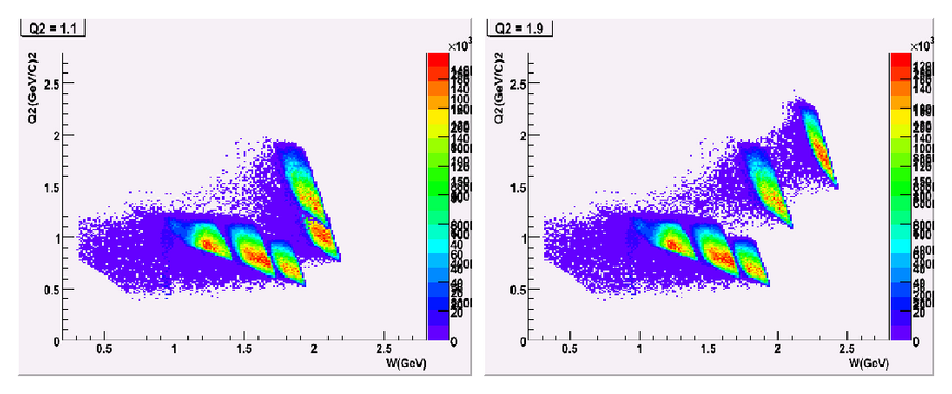
\includegraphics[width=1.0\textwidth]{DW/res_kine.eps}
  \caption{Kinematics coverage of the four resonance measurements}\label{fig:reskine}
\end{figure}

\begin{table}[!htp]
  \begin{center}
    \begin{tabular}{c|c|c|c|c}
      \hline
      $Kine\#$   &   $E_b$    &    $<Q^2>$   &   $<W>$   &   $A_{PV}$ \\
                 &   $GeV$    &    $GeV^2$   &   $GeV$ &   $ppm$   \\
      \hline
      3\*        &    $4.8$   &              &         &
      $-66.3\pm 7.8(stat.)$ \\ 
      4          &    $4.8$   &              &         &   $-73.4\pm 6.9(stat.)$ \\ 
      5          &    $4.8$   &              &         &   $-60.9\pm 5.2(stat.)$ \\ 
      7          &    $6.0$   &              &         &   $-118.8\pm 16.9(stat.)$ \\ \hline
      \end{tabular}
  \end{center}
  \caption{Asymmetry results of the resonance measurements.}\label{tab:resasym}
\end{table}

